\author{João Gonçalves}
\newcommand{\authorr}{Teresa Nogueira}
\newcommand{\authorrr}{André Teodósio}
\newcommand{\authorrrr}{Francisco Carvalho}
\newcommand{\studentID}{99995}
\newcommand{\studentIDD}{100029}
\newcommand{\studentIDDD}{99889}
\newcommand{\studentIDDDD}{99941}
%\newcommand{\supervisorone}{Prof\textsuperscript{\underline{a}}. XXXXXX}
\newcommand{\supervisorone}{João Silvestre}
\newcommand{\supervisortwo}{}
\newcommand{\department}{Engenharia Eletrotécnica e de Computadores}
\newcommand{\exam}{Modelação e Simulação}

\title{%
Trabalho 1\\
\large Modelação de um sistema de terapia de cancro}
\date{Dezembro 2022}

\documentclass[a4paper,12pt]{article}
\usepackage[left=30mm,top=25mm,right=30mm,bottom=25mm]{geometry}
\usepackage[bottom]{footmisc}
\usepackage{etoolbox}
\usepackage{pgfplots}
\usepackage{circuitikz}
\usepackage{booktabs}
\usepackage[usestackEOL]{stackengine}
\usepackage[T1]{fontenc}
\usepackage[utf8]{inputenc}
\usepackage{bm}
\usepackage[export]{adjustbox}
\usepackage{graphicx}
\usepackage[font=footnotesize]{caption}
%\usepackage{caption}
\usepackage{subcaption}
\usepackage{amsmath}
\usepackage{amsfonts}
\usepackage{mathtools}
\usepackage{float}
\usepackage[linktoc=all]{hyperref}
\usepackage[capitalise]{cleveref}
\usepackage{enumitem,kantlipsum}
\usepackage[square,numbers,sort]{natbib}
\usepackage[ruled,vlined]{algorithm2e}
\usepackage{listings}
\usepackage[numbered,framed]{matlab-prettifier}
\usepackage{minted}
\usepackage{amssymb}
\usepackage{babel}
\usepackage[nottoc,numbib]{tocbibind}
\usepackage{tcolorbox}
\usepackage{xcolor}
\usepackage{graphicx,array}
\usepackage{breakurl}
\usepackage{placeins}
\usepackage{colortbl}
\usepackage{attrib}
\usepackage{wrapfig}
\usepackage{mathabx}
\usepackage{fancyhdr}
\usepackage{amsmath}
%\tcbuselibrary{skins,breakable}
%\usetikzlibrary{shadings,shadows}
\usemintedstyle{emacs}
\linespread{1}
%\setlength{\parindent}{0pt}

\newenvironment{block}[1]{%
    \tcolorbox[beamer,%
    noparskip,breakable,
    colback=LightBlue,colframe=DarkBlue,%
    colbacklower=DarkBlue!75!LightBlue,%
    title=#1]}%
    {\endtcolorbox}

\hypersetup{
    colorlinks,
    linkcolor={black},
    citecolor={blue!50!black},
    urlcolor={blue!80!black}
}

\lstset{
  style              = Matlab-editor,
  basicstyle         = \scriptsize\mlttfamily,
  escapechar         = ",
  mlshowsectionrules = true,
  extendedchars=true,
  literate= {á}{{\'a}}1 {é}{{\'e}}1 {í}{{\'i}}1 {ó}{{\'o}}1 {ú}{{\'u}}1 {ç}{{\c c}}1 {ã}{{\~a}}1 {õ}{{\~o}}1
  {Á}{{\'A}}1 {É}{{\'E}}1 {Í}{{\'I}}1 {Ó}{{\'O}}1 {Ú}{{\'U}}1 {Ã}{{\~A}}1,
}

\def\delequal{\mathrel{\ensurestackMath{\stackon[1pt]{=}{\scriptstyle\Delta}}}}
%------------------------------------ MAGIC--------------------------------------
\def\UrlBreaks{\do\/\do-}
\expandafter\def\expandafter\UrlBreaks\expandafter{\UrlBreaks\do\a%
\do\b\do\c\do\d\do\e\do\f\do\g\do\h\do\i\do\j\do\k\do\l\do\m\do\n%
\do\o\do\p\do\q\do\r\do\s\do\t\do\u\do\v\do\w\do\x\do\y\do\z\do\&}

\newcolumntype{C}[1]{>{\centering\let\newline\\\arraybackslash\hspace{0pt}}m{#1}}
\newcolumntype{L}[1]{>{\raggedright\let\newline\\\arraybackslash\hspace{0pt}}m{#1}}
%----------------------------------TITLE PAGE -----------------------------------
\makeatletter
\def\maketitle{
  \begin{center}\leavevmode
        \normalfont
        
\includegraphics[width=0.5\columnwidth]{img/title-page/IST.pdf}
        \vskip 0.05cm   
        \textsc{\large \department}\\
        \vskip 0.5cm
        \rule{0.95\linewidth}{0.2 mm} %\\
        {\large \exam}\\[0.5 cm]
        {\huge \bfseries \@title \par} 
        
\includegraphics[scale=0.65]{img/title-page/-000.jpg}
        \vspace{-2em}
        \captionof*{figure}{\color{gray} Imagem: freepik.com}
        %\vspace{0.5cm}
        \rule{0.95\linewidth}{0.2 mm} \\[0.75 cm]
        %\fontsize{9pt}{11pt}\selectfont
        \begin{minipage}[t]{0.45\textwidth}
	    \begin{flushleft} \large
                \emph{Autores:}\\
		    \normalsize \textbf{\authorrr} : \studentIDDD\\
                \scriptsize $\hookrightarrow$ andre.teodosio@tecnico.ulisboa.pt \\
                \normalsize \textbf{\authorrrr} : \studentIDDDD \\
                \scriptsize $\hookrightarrow$ franciscosoaresc@tecnico.ulisboa.pt
            \end{flushleft}
	\end{minipage}
        \begin{minipage}[t]{0.45\textwidth}
	   \begin{flushleft} \large
                \vphantom{teste 123} \\
			\normalsize \textbf{\@author} : \studentID\\
                \fontsize{9pt}{11pt}\selectfont $\hookrightarrow$ jrazevedogoncalves@tecnico.ulisboa.pt \\
                \normalsize \textbf{\authorr} : \studentIDD\\
                \scriptsize $\hookrightarrow$ maria.teresa.ramos.nogueira@tecnico.ulisboa.pt
		\end{flushleft}
	\end{minipage}
        \vskip 1em
        \begin{minipage}[t]{0.45\textwidth}
	   \begin{flushleft} \large
			\ifdefempty{\supervisortwo}{\emph{Docente:\\}}{\emph{Supervisores:\\}}
			\supervisorone\\
			\ifdefempty{\supervisortwo}{}{\supervisortwo\\}
		\end{flushleft}
	\end{minipage}
         \begin{minipage}[t]{0.45\textwidth}
	   \begin{flushright} \large
			\phantom{123 experiência}
		\end{flushright}
	\end{minipage}
        \vspace{0.35cm}
        \begin{quotation}
            \textit{O grupo de alunos acima identificado garante que o texto deste relatório e todo o software e resultados entregues foram inteiramente realizados pelos elementos do grupo, com uma participação significativa de todos eles, e que nenhuma parte do trabalho ou do software e resultados apresentados foi obtida a partir de outras pessoas ou fontes.}
        \end{quotation}
	\vfill
	{\Large \@date\par}
   \end{center}
   %\vfill
   %\null
   \cleardoublepage
  }
\makeatother
%-------------------------------- ENDTITLE PAGE ----------------------------------
%---> Header <---
%\fancyhf{}
\renewcommand{\headrulewidth}{1pt}% Header rule width
\renewcommand{\footrulewidth}{0pt}% No footer rule
\setlength\headheight{26pt} 
\fancyhead[L]{\raisebox{0.1\height}[0pt][0pt]{\textit{Modelação e Simulação}}}
\fancyhead[R]{\raisebox{0.1\height}[0pt][0pt]{2022/2023}}

\pgfplotsset{compat=1.18}
\setcounter{tocdepth}{4}
%\setcounter{secnumdepth}{4}
\setcounter{secnumdepth}{-2}
\setlength{\bibsep}{0.1em}%reduzir espaço entre refs.

\newtheorem{theorem}{Theorem}[section]
\graphicspath{{figures/}}

\renewcommand{\figurename}{Fig.}
\renewcommand{\tablename}{Tab.}
\renewcommand{\contentsname}{Índice}
\settocbibname{Referências}

\begin{document}
    \sloppy
    %% title page
    \pagenumbering{gobble}
    \pagestyle{empty}
    \maketitle

    \newgeometry{left=25mm,top=23.5mm,right=25mm,bottom=23.5mm}
    %% toc
    %\tableofcontents
    %% body
    \newpage
    \pagestyle{fancy}
    \pagenumbering{arabic}
    %\section{Perguntas}
    \phantomsection\addcontentsline{toc}{section}{Perguntas}\vskip -0em%
        %//==============================--@--==============================//%
\vspace{-1em}
\subsection{P1 | Simulação do modelo PK (método de Euler)}
\label{subsec:P1}

\vskip -1.5em
\begin{wrapfigure}{l}{0.3\textwidth}
    \centering
    
\includegraphics[width=0.275\textwidth]{img/perguntas/P1/P1-modelo-compartimental.png}
    \caption{Modelo compartimental \textcolor{gray}{(Imagem: Guia Laboratorial)}.}
    \label{fig:P1-modelo-compartimental}
\end{wrapfigure}

\vphantom{1}

A farmacocinética (PK) é responsável por determinar o destino das substâncias administradas no organismo e, portanto, os perfis\footnotemark[1] de tempo de concentração de substâncias no corpo. 

Tomando uma \textit{mechanistic modeling}\cite{teles_2017}, consideramos o modelo PK exposto (constantes definidas no Guia\scalebox{0.7}{$^{*^**}$}):
\vspace{-0.35em}\begin{equation}
    \begin{bmatrix}
        \dot{c_1} \\
        \dot{c_2}
    \end{bmatrix} =
    \begin{bmatrix}
        \frac{1}{V_1}(-K_{12}-K_{10}) & \frac{1}{V_1}K_{21}\\
        \frac{1}{V_2}K_{12} & -\frac{1}{V_2}K_{21}
    \end{bmatrix}
    \begin{bmatrix}
        c_1\\
        c_2
    \end{bmatrix} +
    \begin{bmatrix}
        \frac{1}{V_1}\\
        0
    \end{bmatrix}\delta d
\end{equation}

%%% BEGIN TABULAR
\vspace{-1em}
\begin{tabular}{c c}%%
    \hspace*{-1em}\noindent\begin{minipage}[t]{0.475\textwidth}
        \begin{lstlisting}[title=Pergunta 1 - Modelo PK (método de Euler),frame=tlrb]{P1}
%% Define variables
% (...)
%% Create f function -> c(t)' = f(c,d)
f = @(c,d)[
    (1/V*(-K12-K10)*c(1,:)+1/V*K21*c(2,:)+delta/V*d);
    (1/V*K12*c(1,:) - 1/V*K21*c(2,:))];
%% P1
Euler(f,t,h,d,size);
function Euler(f,t,h,d,size)
    % Preallocation
    c = zeros(2,size-1); 
    % Simple Euler's integration
    for i = 1:(size-1)
        c(:,i+1) = c(:,i) + h*f(c(:,i),d(i));
    end
    % Plot PK
    figure(), plot(t,c(1,:)), hold on; 
    plot(t,c(2,:)), plot(t,d);
    % (...)
end
        \end{lstlisting}
    \end{minipage} &\
    \noindent\begin{minipage}[t]{0.5\textwidth}
        \begin{figure}[H]
            \hspace*{-1.25em}
            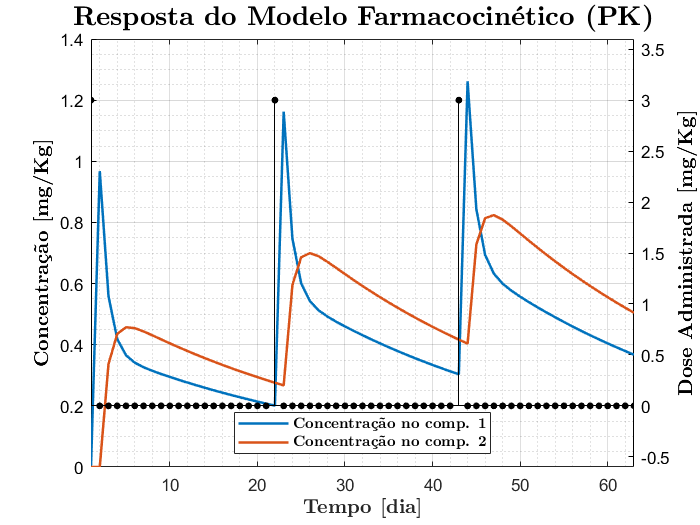
\includegraphics[width = 1\linewidth]{img/perguntas/P1/P1-PK.png}
            \caption{Concentrações nos compartimentos \textcolor{blue}{1} e \textcolor{orange}{2},\\ e dose administrada com um período de $T=21$d.}
            \label{fig:P1-modelo-PK}
        \end{figure}
    \end{minipage}
\end{tabular}
%%% END TABULAR

\vspace{1em}
Verifica-se que a administração de uma dose do fármaco, aumenta rapidamente $c_1$, correspondendo à \underline{fase de absorção} do medicamente pelo organismo. Em seguida,  observa-se a \underline{fase de distribuição}, em que a substância é distribuída ao longo do corpo, entranhando-se na(s) zona(s) de atuação, o que corresponde à diminuição de $c_1$ e aumento de $c_2$. Esta variação é proeminente logo após a administração, uma vez que a diferença de concentrações se verifica mais acentuada. A terceira fase observada corresponde à \underline{fase de excreção/metabolismo} do organismo, onde ambas as concentrações diminuem.
%//==============================--@--==============================//%
\footnotetext[1]{Estes perfis dependem de uma panóplia de fatores relacionados com propriedades da substância e à forma como o organismo reage inerentemente a esta; bem como do método de administração.\cite{teles_2017}}

        %\clearpage
%//==============================--@--==============================//%
\subsection{P2 | Efeito do fármaco em função da dose (modelo PD)}
\label{subsec:P2}

A farmacodinâmica (PD) permite descrever a relação\footnotemark[2] entre o efeito de um fármaco ($u$) e a sua concentração ($C_p$) no compartimento de efeito. O modelo PD é amplamente representado pela equação de Hill\cite{Goutelle2008-bv}:

\vspace{-1em}
\begin{equation}\label{eq:modelo-PD}
    u \delequal u_{max}\frac{C^\alpha_p(t)}{C^\alpha_{50} + C^\alpha_p(t)}
\end{equation}
onde $u_{max}$ é o efeito máximo do fármaco (tipicamente um valor unitário\cite{teles_2017}), $C_{50}$ a concentração para qual 50\% do efeito máximo é obtido\footnotemark[3], e $\alpha$ denota o coeficiente de Hill que determina a \textit{steepness} da sigmoide resultante.
%//==============================--@--==============================//%
\footnotetext[2]{Contribui para a compreensão da resposta medicamentosa e da sua eficácia.}
\footnotetext[3]{Considera-se $C_{50} = 7.1903$ mg/kg (Atezolizumab)\protect\cite{belfo_2018}\cite{teles_2017}.}
%//==============================--@--==============================//%
\newpage
\vskip -1em
\begin{wrapfigure}{l}{0.5\textwidth}
    \centering
    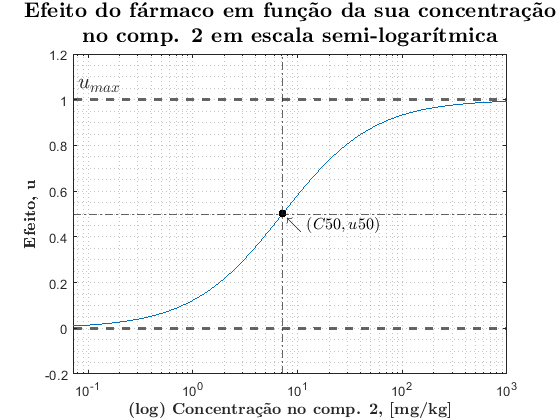
\includegraphics[width=0.5\textwidth]{img/perguntas/P2/P2-Hill.png}
    \caption{Efeito do fármaco em função de $C_p$ em escala semi-logarítmica\protect\footnotemark[4] (com os níveis de saturação salientados), para $\alpha = 1$, $u_{max} = 1$ e $C_{50} = 7.1903$ ($\pmb{\star}$ \textbf{valores considerados ao longo do relatório}).}
    \label{fig:P2-Hill}
\end{wrapfigure}

Como explicitado na \hyperref[fig:P2-Hill]{Fig. 2}, a equação de Hill introduz uma saturação na variação da concentração do fármaco. 

Tal traduz-se em concentrações baixas, resultarem em efeitos bastante diminutos; e concentrações elevadas, tenderem para um efeito saturado, i.e., $\pmb{\star}$ \textbf{administrações com dosagens \underline{mais elevadas} do que um certo patamar, \underline{não produzem} um maior efeito na redução do tumor}.

Para além disto, há que ter em consideração a carga tóxica a que o organismo é exposto na terapia, o que torna a dosagem num parâmetro de fulcral controlo, proeminentemente com fármacos de elevada toxicidade. Acrescenta-se:

\vphantom{Experiência 123}

\vspace{-1.5em}
\begin{quote}
    ``\textit{O que é que não é um veneno? Todas as coisas são veneno e nada é sem veneno. Somente a dose determina que algo não seja um veneno.}''
    
    \attrib{Paracelso}
\end{quote}

\vspace{-1.5em}
\begin{wrapfigure}[16]{l}{0.5\textwidth}
    \centering
    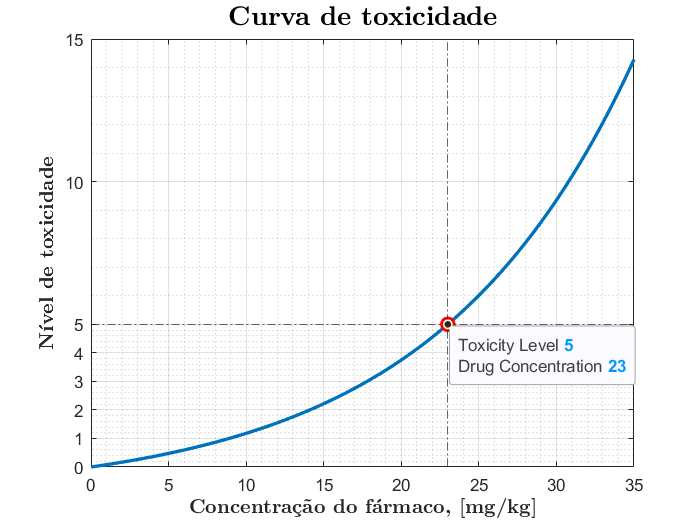
\includegraphics[width=0.5\textwidth]{img/perguntas/P2/P2-toxicity.png}
    \caption{Níveis de toxicidade para o fármaco Atezolizumab. A marca representa a concentração para qual o nível de toxicidade é máximo (\textit{grade} 5).}
    \label{fig:P2-toxicity}
\end{wrapfigure}

\vphantom{1}
\vskip 0.25em
No entanto, os níveis de toxicidade não podem ser explicitamente aferidos\footnotemark[5] e não existem modelos para esta avaliação\cite{teles_2017}.

Ao estudar a concentração de um fármaco no organismo durante uma terapia, é possível estimar os níveis de toxicidade ``\textit{by using a function yielding a certain small value until a certain amount of concentration is achieved. After this threshold, the function grows exponentially}\cite{toxicity-lemos}.''\cite{teles_2017} A \hyperref[fig:P2-toxicity]{curva de toxicidade} foi escolhida de modo a que a \textit{morte}\footnotemark[5] seja atingida quando a concentração do fármaco no organismo excede por 15\% o maior valor de dose permissível\footnotemark[6].
%//==============================--@--==============================//%
\footnotetext[4]{"The semi-log plot is the preferred method for plotting concentration-response relationships because it becomes easier to accurately determine the EC50 value (...) by placing it on a linear portion (...)"\cite{Salahudeen2017-pb}}

\footnotetext[5]{Não obstante, o \textit{Common Terminology Criteria for Adverse Events} (CTCAE) permite classificar a toxicidade em ensaios clínicos como:\\
$\xrightarrow[]{}$ leve (\textit{grade} 1), moderada (\textit{grade} 2), severa (\textit{grade} 3), risco de morte (\textit{grade} 4) e morte (\textit{grade} 5).}

\footnotetext[6]{Para o fármaco Atezolizumab $\xrightarrow[]{}$ 20 mg/kg\cite{Fu_undated-zm}.}
        %//==============================--@--==============================//%
\subsection{P3 | Modelo de crescimento do tumor}
\label{subsec:P3}
%//==============================--A--==============================//%
\vspace{-0.5em}
\subsubsection[a) Pontos de equilíbrio]{a) Pontos de equilíbrio (para $u = 0$)}% 'TeX não gosta de math nos títulos, nifty trick
\label{subsubsec:P3a}

No equilíbrio, $V(t)$ é constante, e consequentemente, a primeira derivada é nula.
\vskip -0.75em
$$
    \begin{cases}
        \dot{V}(t) = 0\\
        u = 0
    \end{cases}\implies
    aV\left(1 - \frac{V}{K_T} \right) = 0 \implies V = 0 \lor V = K_T = 10\ \text{mm}^3
$$
%//==============================--B--==============================//%
\subsubsection[b) Análise da monotonia da variável V (para u = 0)]{b) Análise da monotonia da variável $V$ (para $u = 0$)}% 'TeX não gosta de math nos títulos, nifty trick
\label{subsubsec:P3b}
\vspace{-1.5em}
\hspace*{-2.25em}
\begin{tabular}{c c}
    \noindent\begin{minipage}[t]{0.5\textwidth}
        \begin{figure}[H]
            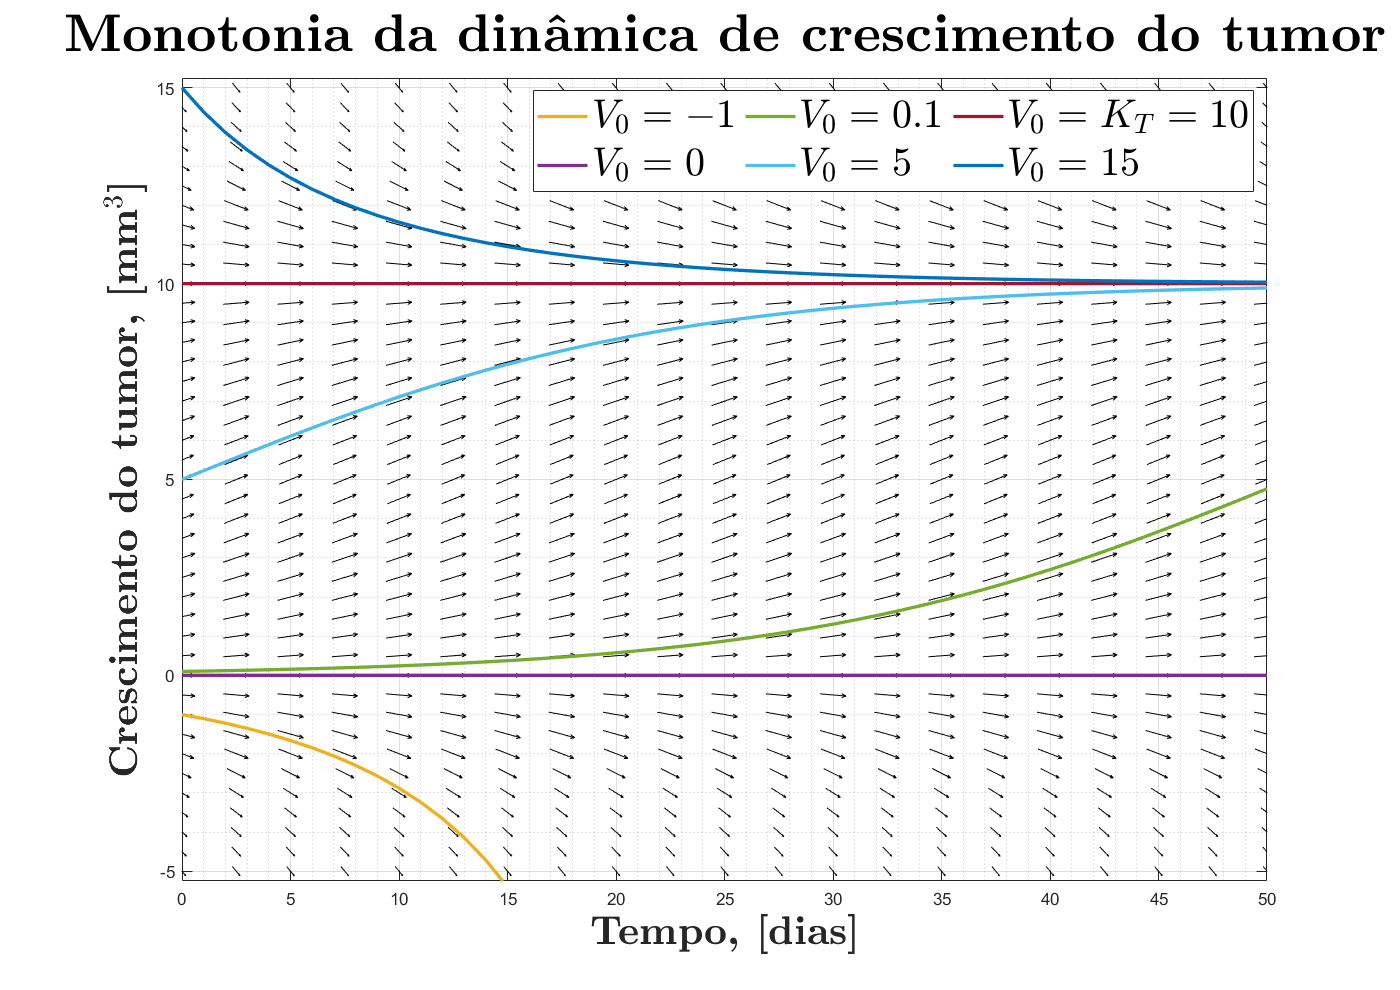
\includegraphics[width = 1\linewidth]{img/perguntas/P3/P3-monotonia.png}
            \hspace*{1.65em}\begin{minipage}{1\linewidth}
                \caption{Evolução do volume do tumor para\\ diferentes valores iniciais.}
                \label{fig:P3-monotonia}
            \end{minipage}
        \end{figure}
    \end{minipage} &\
    \hspace*{-1em}\noindent\begin{minipage}[t]{0.5\textwidth}
            \vspace{1.75em}
            \hspace*{1.35em}\begin{minipage}{1\linewidth}
                \captionof{table}{Tabela de monotonia do crescimento\\ do tumor $V(t)$ para $u = 0$.}
                \label{tab:P3-monotonia}
            \end{minipage}
            \renewcommand\arraystretch{1.5}
            \hspace*{-0.5em}\begin{tabular}{*{8}{c}}
                \toprule
                $V(t)$ & $-\infty$ & & $0$ & & $K_T$ & & $+\infty$ \\
                \midrule
                $\dot{V}(t)$ & $-$ & $-$ & 0 & $+$ & 0 & $-$ & $-$ \\
                %$\Ddot{V}(t)$ & $-$ & $-$ & 0 & $+$ & 0 & $-$ & $-$ \\
                $V(t)$ & \multicolumn{2}{c}{$\color{blue} \pmb{\searrow}$} & $eq_{min}$ & $\color{blue} \pmb{\nearrow}$ & $eq_{max}$ & \multicolumn{2}{c}{$\color{blue} \pmb{\searrow}$} \\
                \bottomrule
            \end{tabular}
            \vspace{0.3em}
            \[ \therefore \text{\textbf{Monotonia de }} V(t) \]
            \[ \raisebox{0.2 em}{$\drsh$}\ \text{\textbf{Decrescente}:}\ V \in\ \left]-\infty, 0\right[\, \cup\, \left]K_T, +\infty\right[ \]
            \vspace{-1.7em}
            \[ \hspace*{-5em} \raisebox{0.2 em}{$\drsh$}\ \text{\textbf{Crescente}:}\ V \in\ \left]0, K_T\right[ \]      
    \end{minipage}
\end{tabular}

Ao iniciar a simulação com um volume de $V_0 = 0$, não há crescimento, e o volume mantém-se em zero. Para um volume inicial de $0<V(t_0)<K_T$, verifica-se então um crescimento; no entanto, é atingido um \textit{plateau}, quando $V(t)$ se aproxima de $K_T$ (\textit{saturation level}/\textit{carrying capacity}). Para $V_0 = K_T$, também não ocorre crescimento, e o volume permanece neste valor (vide a \hyperref[subsubsec:P3a]{secção anterior}). Finalmente, se começarmos com um volume superior a $K_T$, o volume decresce até eventualmente se encontrar na vizinhança da solução de equilíbrio assintóticamente estável.

Note-se que foi incluída uma secção de $V$'s negativos (apesar de não ter qualquer significado num contexto real), de modo a explicitar o comportamento "perto" de $V_0 = 0$ (solução de equilíbrio assintóticamente instável).

%//==============================--C--==============================//%
\subsubsection[c) Poderá V assumir valores negativos mediante valores de u?]{c) Poderá $V$ assumir valores negativos mediante valores de $u \in [0; 1]$?}% 'TeX não gosta de math nos títulos, nifty trick 
\label{subsubsec:P3c}
Seja $0 \leq u(t) \leq u_{max}$ e $V(t_0) > 0$. Tendo em conta a equação logística:
\vspace{-0.25em}
\begin{equation}
    \dot{V}(t) = aV\left(1-\frac{V}{K_T}\right) - buV = \left[ a\left( 1-\frac{V}{K_T} \right) - bu \right]V = [a-bu]V-\left[\frac{a}{K_T}\right]V^2
\end{equation}

\vspace{-0.25em}
\noindent verifica-se que os \underline{pontos de equilíbrio} passam a ser:
\vspace{-0.75em}
$$
    V = 0\quad\lor\quad V = \chi \delequal K_T-\frac{buK_T}{a}
$$
\vspace{-2.25em}
%\iffalse
\begin{figure}[!h]
    \centering
    \begin{subfigure}[b]{0.25\textwidth}
    \centering
    \resizebox{1\textwidth}{!}{%
        \begin{tikzpicture}
            \begin{axis}[
                axis lines = center,
                xlabel = {$V(t)$},
                ylabel = {$\dot{V}(t)$},
                y label style={at = {(0.13,1.00575)}},
                grid style=dashed,
                grid=none,
                ticks=none
            ]

            \addplot[
                domain=(-3):(7), 
                samples=300, 
                color=darkgray,
                dashed
            ]
            {-x*(x-4)};

            % pontos
            \node[label={55:{\color{darkgray} $\pmb{\chi}$}},inner sep=2pt] at (3.4,-3) {};
            \node[label={55:{\color{darkgray} $\pmb{0}$}},inner sep=2pt] at (0,-3) {};

            % signs
            \node[label={0:{\color{red} $\pmb{-}$}},inner sep=2pt] at (5.2,-5.8) {};
            \node[label={0:{\color{red} $\pmb{-}$}},inner sep=2pt] at (-2.2,-5.8) {};
            \node[label={0:{\color{red} $\pmb{+}$}},inner sep=2pt] at (1.5,1.65) {};

            % arrows
            \draw[->] (axis cs:3.3, 3.7) -- (axis cs:4.2, 0.7);
            \draw[->] (axis cs:5.1, -3.7) -- (axis cs:4.55, -0.7);
            
            %\addlegendentry{}
            \end{axis}
        \end{tikzpicture}
    }%
    \caption{Caso com $u \in [0, 0.09[$}
    \end{subfigure}\qquad
    \begin{subfigure}[b]{0.25\textwidth}
    \centering
    \resizebox{1\textwidth}{!}{%
        \begin{tikzpicture}
            \begin{axis}[
                axis lines = center,
                xlabel = {$V(t)$},
                ylabel = {$\dot{V}(t)$},
                y label style={at = {(0.35,1.005)}},
                grid style=dashed,
                grid=none,
                ticks=none,
                ymax=1.9,
                ymin=-10
            ]

            \addplot[
                domain=(-15):(15), 
                samples=300, 
                color=darkgray,
                dashed
            ]
            {-x^2};

            % pontos
            \node[label={55:{\color{darkgray} $\pmb{0 \equiv \chi}$}},inner sep=2pt] at (0,-0.25) {};

            % signs
            \node[label={0:{\color{red} $\pmb{-}$}},inner sep=2pt] at (1.7,-2.3) {};
            \node[label={0:{\color{red} $\pmb{-}$}},inner sep=2pt] at (-2.4,-2.3) {};

            % arrows
            \draw[->] (axis cs:1.5, -1.7) -- (axis cs:1, -0.5);

            %\addlegendentry{}
            \end{axis}
        \end{tikzpicture}
    }%
    \caption{Caso com $u = a = 0.09$}
    \end{subfigure}\qquad
    \begin{subfigure}[b]{0.25\textwidth}
    \centering
    \resizebox{1\textwidth}{!}{%
        \begin{tikzpicture}
            \begin{axis}[
                axis lines = center,
                xlabel = {$V(t)$},
                x label style={at = {(1,0.7)}},
                ylabel = {$\dot{V}(t)$},
                grid style=dashed,
                grid=none,
                ticks=none
            ]

            \addplot[
                domain=(-7):(3), 
                samples=300, 
                color=darkgray,
                dashed
            ]
            {-x*(x+4)};

            % pontos
            \node[label={55:{\color{darkgray} $\pmb{\chi}$}},inner sep=2pt] at (-4.3,-3) {};
            \node[label={55:{\color{darkgray} $\pmb{0}$}},inner sep=2pt] at (-0.8,-3) {};

            % signs
            \node[label={0:{\color{red} $\pmb{-}$}},inner sep=2pt] at (1.2,-5.8) {};
            \node[label={0:{\color{red} $\pmb{-}$}},inner sep=2pt] at (-6.2,-5.8) {};
            \node[label={0:{\color{red} $\pmb{+}$}},inner sep=2pt] at (-2.5,1.65) {};

            % arrows
            \draw[->] (axis cs:1.1, -3.7) -- (axis cs:0.5, -0.7);

            %\addlegendentry{}
            \end{axis}
        \end{tikzpicture}
    }%
    \caption{Caso com $u \in\ ]0.09, 1]$}
    \end{subfigure}
\caption{Comportamento de $\dot{V}$ em função de $V$. A \textcolor{red}{vermelho} encontra-se o sinal de $\dot{V}$ que rege a monotonia de $V$ (para o caso específico). O ponto de equilíbrio $\chi$ modifica-se consoante $u$. Este comportamento, modifica a estabilidade dos pontos de equilíbrio (vide os \textcolor{red}{sinais} da derivada para os casos distintos). Em \hyperref[fig:P3-c]{(a)} verifica-se um caso semelhante à \hyperref[subsubsec:P3b]{alínea b)}, em que $\chi$ é o ponto de equilíbrio estável (i.e., $\forall V_0>0: V \xrightarrow{} \chi$). Para os casos explícitos em \hyperref[fig:P3-c]{(b)} e \hyperref[fig:P3-c]{(c)}, dado que $V(t_0)>0$, após a análise gráfica\protect\footnotemark[7] (e dos \textcolor{red}{sinais} de $\dot{V}$), trivialmente se conclui que as soluções tendem \underline{sempre} para $0$ (nunca o ultrapassando) para $u \in [0.09, 1]$.} \label{fig:P3-c} 
\end{figure}
%\fi
%//==============================--@--==============================//%
\vspace{-1em}\footnotetext[7]{As setas representadas nas \hyperref[fig:P3-c]{figuras} explicitam o movimento intuitivo (consoante o \textcolor{red}{sinal} da derivada) de $V$ (somente para $V(t_0)>0$, dada a relevância) em relação às soluções de equilíbrio assintóticas.}
        \clearpage
%//==============================--@--==============================//%
%\vspace{-1em}
\subsection{P4 | Simulação do sistema completo}
\label{subsec:P4}
%//==============================--A--==============================//%
\vspace{-0.5em}
\subsubsection{a) Gráficos das variáveis relevantes}
\label{subsubsec:P4a}

%%% 
\vspace{-1em}
\noindent\begin{minipage}[t]{0.45\textwidth}
\begin{lstlisting}[title=Pergunta 4, frame=tlrb]{P4-a}
%% Function calls

% init concentration
c = concentration(); % same function as in P1

% init effect
u = Hill(c);
% init volume growth
v = Tumor(u);
% plot
PlotRelevantVariables(c, d, v, u);
%%
function v = Tumor(u)
    %tumor growth variables 
    a = 0.09; b = 1; Kt=10; h = 1; p0 = 1; %1mm^3 
    size = length(u);
\end{lstlisting}
\end{minipage}
\hfill \noindent\begin{minipage}[t]{0.45\textwidth}
\begin{lstlisting}[title = (continuação), frame=tlrb]{P4-a}
    %create logistic equation
    l = @(v,u)a*v*(1-v./Kt) - b*u.*v;
    %preallocating for speed
    v = zeros(1,size); v(1) = p0; %<- v0
    %simple Euler's integration
    for i = 1:(size - 1)
        v(i+1) = v(i) + h*l(v(i),u(i));
    end
end
%%
function u = Hill(c)
    %half maximal effect
    c50 = 7.1903;
    %create Hill's equation: Pharmacodynamic model
    u = c(2,:)./(c50 + c(2,:));
end
\end{lstlisting}
\end{minipage}

\vspace{1em}
 \hspace*{-1.98cm}\begin{tabular}{C{9cm}  L{8 cm}}
        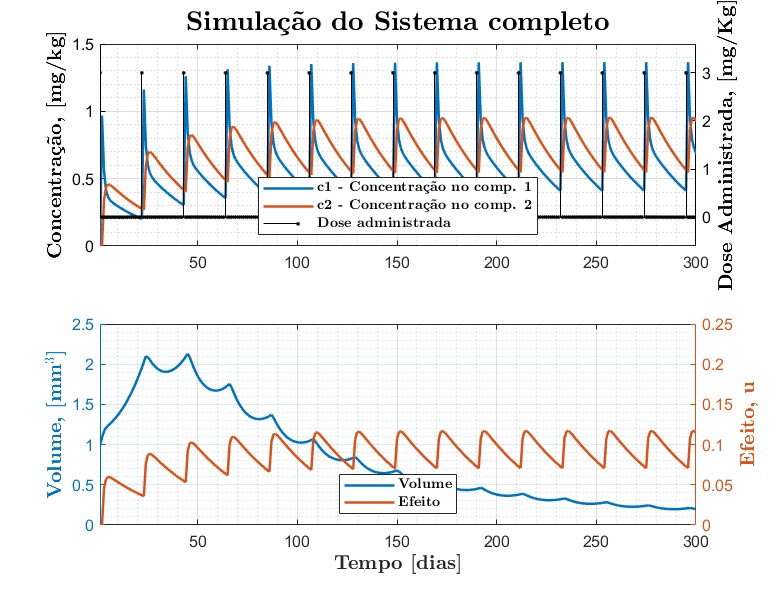
\includegraphics[width=\linewidth]{img/perguntas/P4/P4-a.png} & 
        \vspace{-2.5em} \captionof{figure}{\textbf{Simulação do sistema completo}.} 
        \vspace{0.5em}
        \hspace*{1em} Procedeu-se à simulação do sistema completo, considerando uma administração equiespaçada de período $T = 21$d (utilizada em alíneas anteriores) mediante uma janela temporal de 300 dias. O tumor, após atingir 200\% do volume inicial, é lentamente erra- dicado, aparente na diminuição de volume com a constante administração do fármaco.
        
        \hspace*{1em} A característica ondulatória da evolução do volume do tumor deve-se à presença reduzida do fármaco no organismo, conse- quência da dosagem de $3$ mg/kg.
    \end{tabular}
%//==============================--B--==============================//%
\subsubsection{b) Otimização do espaçamento entre aplicações do fármaco}
\label{subsubsec:P4b}
%%% BEGIN TABULAR
\vspace{-1em}
\begin{tabular}{c c}%%
    \hspace*{-1em}\noindent\begin{minipage}[t]{0.475\textwidth}
\begin{lstlisting}[title=Pergunta 4 - Aquisição do espaçamento,frame=tlrb]{P4-b}
function T = Optimal()
    %declare requerimen
    opVolume = 0.10; N = 25; d = zeros(1,N) + 3;
    
    for T = 1:21
        clear dosage; dosage = upsample(d,T); 

        % Calculate volume evolution
        c = concentration(dosage);
        u = Hill(c);
        v = Tumor(u);

        % evaluate volume at 25 day mark
        if v(25) >= opVolume
            break
        end
    
    end
    fprintf("Optimal periodicity: \%i days\textbackslash n", T);
    
end
\end{lstlisting}
    \end{minipage} &\
    \noindent\begin{minipage}[t]{0.5\textwidth}
        \begin{figure}[H]
            \vspace{-0.4em}
            \hspace*{-1.25em}
            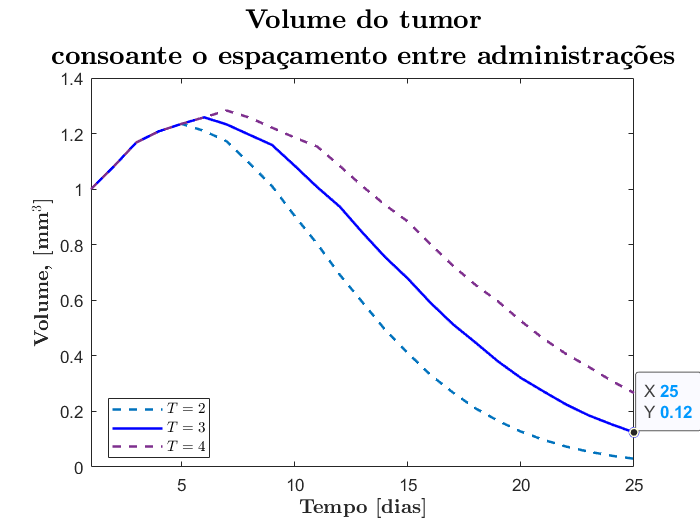
\includegraphics[width = 1\linewidth]{img/perguntas/P4/P4-b.png}
            \caption{Evolução do volume do tumor consoante 3 espaçamentos adjacentes. A \textcolor{blue}{azul} verifica-se a curva com o valor ótimo para solucionar os requerimentos.}
            \label{fig:P4-b}
        \end{figure}
    \end{minipage}
\end{tabular}
%%% END TABULAR

%//==============================--@--==============================//%

        \clearpage
%//==============================--@--==============================//%
\subsection{P5 | Espaçamento variável entre as tomas de medicamento}
\label{subsec:P5}
O espaçamento variável depende do objetivo do modelo de tratamento proposto, nomeadamente, \textbf{erradicação} ou \textbf{supressão} do tumor:
%//==============================--I--==============================//%
\vspace{-1em}
\subsubsection{$\pmb{\xrightarrow[]{}}$ \textit{Front-Load dosing}}
\label{subsubsec:front-load-dosing}
\vspace{-2.5em}
\hspace*{-0cm}\begin{wrapfigure}[11]{l}{0.5\textwidth}
    \centering
    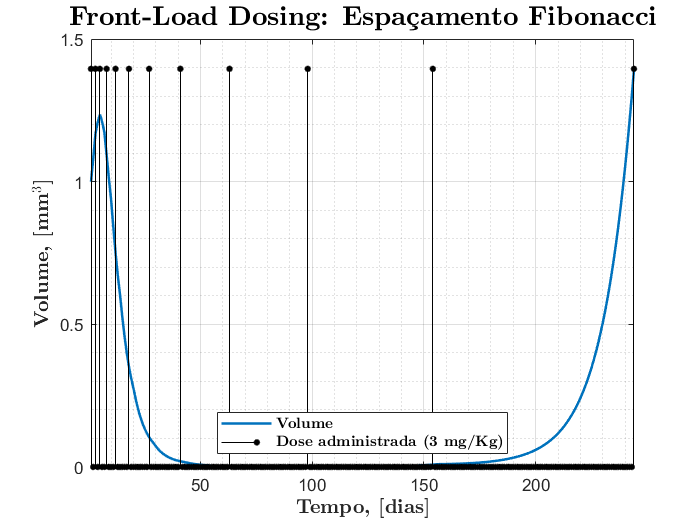
\includegraphics[width=0.5\textwidth]{img/perguntas/P5/P5-Fib.png}
    \vspace{-0.1em}\begin{minipage}{1\linewidth}
        \caption{Simulação da administração \textit{Front-Load} mediante a sequência de Fibonacci.}
        \label{fig:P5-fib}
    \end{minipage}
\end{wrapfigure}

\begin{quote}
     \textit{``Dosing by ``front-loading'' has thus become the mainstay of treatment, owing largely to theoretical and laboratory studies over the past 40 years (...)''}\cite{Hahnfeldt2003-oy}
\end{quote}

\textbf{Front-Loading} $\rightarrow$ Administração de doses elevadas de fármaco mediante espaçamentos de curta duração na fase inicial de terapia.

\vphantom{esperiencia123}

\vphantom{esperiencia123}

\vphantom{esperiencia123}

A administração \textit{Front-Load} procura \underline{erradicar} o tumor nos estágios iniciais de desenvolvimento, evitando aquisições elevadas de resistência (vide \hyperref[subsec:P6]{secção P6}). A simulação evidencia uma rápida diminuição do volume cancerígeno com aproximação do limite assíntótico em $V = 0$ na marca dos 50 dias e ainda um baixo crescimento máximo de 23\% do volume inicial (5º. dia). 

Em contexto real, esta impressionante diminuição de volume\footnotemark[7] revela-se inconsistente: a remissão é muitas vezes seguida de reincidência (de forma análoga ao crescimento na marca dos 150 dias, na \hyperref[fig:P5-fib]{Fig. 9})\footnotemark[8]. Esta administração apresenta alguns pontos pouco favoráveis:
\vspace{-0.75em}
\begin{enumerate}
    \itemsep 0em 
    \item Aplicação de uma elevada dose de fármaco num curto espaço de tempo leva a um incremento da carga tóxica no corpo hospedeiro (vide \hyperref[subsec:P2]{secção P2}).
    \vspace{-0.5em}\item Dificuldade em limitar a ação do fármaco ao tumor: \textit{``threat to the bone marrow and other at-risk stem cell compartments.''}\cite{Hahnfeldt2003-oy}
    \vspace{-0.5em}\item Eficácia reduzida em massas cancerígenas heterogéneas (\textit{``The cell population subject to treatment is in general not uniform, consisting instead of sensitive and resistant subpopulations.''})
\end{enumerate}

%//==============================--II-==============================//%
\vspace{-2em}
\subsubsection{$\pmb{\xrightarrow[]{}}$ \textit{Metronomic dosing}}
\label{subsubsec:metronomic-dosing}
\begin{quote}
    ``\textit{Recently, a revolutionary form of chemotherapy has emerged. Metronomic chemotherapy (...)}''\cite{elisa_2017}
\end{quote}
A administração metronómica depende de uma administração continua e periódica de baixa dosagem (\textit{minimum biologically effective dose}\cite{elisa_2017}) e consequentemente de baixa toxicidade, sem períodos de pausa entre fases de administração (\textit{no prolonged drug-free breaks}\cite{elisa_2017}). Esta administração não procura erradicar mas sim \underline{suprimir} o tumor: \textit{``Patient survival is not incompatible with tumor presence.''}\cite{Hahnfeldt2003-oy}.

Este modelo de espaçamento preenche as lacunas do anterior:

\vphantom{esperiencia123}
\begin{enumerate}
    \itemsep 0em 
    \vspace{0em}\item Aplicação de baixas doses de fármaco, que por consequência, não excedem a dose permissível deste no organismo (\hyperref[subsec:P2]{secção P2}).
    \vspace{-0.5em}\item  Permite a restauração de células essenciais (\textit{``stemcell recovery''}\cite{Hahnfeldt2003-oy}).
    \vspace{-0.5em}\item  Limita a proliferação de células resistentes através da manutenção de uma elevada proporção de células sensíveis no seio do tumor: \textit{``due to competition for space and resources between these populations (...)''}\cite{elisa_2017}  $\xrightarrow[]{}$ \textit{Resensitization effect}\cite{Hahnfeldt2003-oy}.
\end{enumerate}

\vspace{-0.5em}
\noindent $\pmb{\star}$ \textbf{São considerados dois casos de espaçamento metronómico:}

%//==============================--II-==============================//%
\footnotetext[7]{Comparativamente à administração abordada \hyperref[subsubsec:P4a]{na secção 4 a)}}
\footnotetext[8]{Embora o recrescimento do tumor na simulação seja resultado da limitação da equação logística (vide \hyperref[subsubsec:P3c]{secção P3 c)}), podemos admitir esta reincidência perto da realidade.}
%//==============================--II-==============================//%
%\clearpage
%//==============================--i--==============================//%
\vspace{-1.5em}\paragraph{i) \textit{Pattern}}\mbox{}\\
\label{subsubsubsec:pattern}
\vspace{-2.5em}
\hspace*{-0cm}\begin{wrapfigure}[12]{l}{0.47\textwidth}
    \centering
    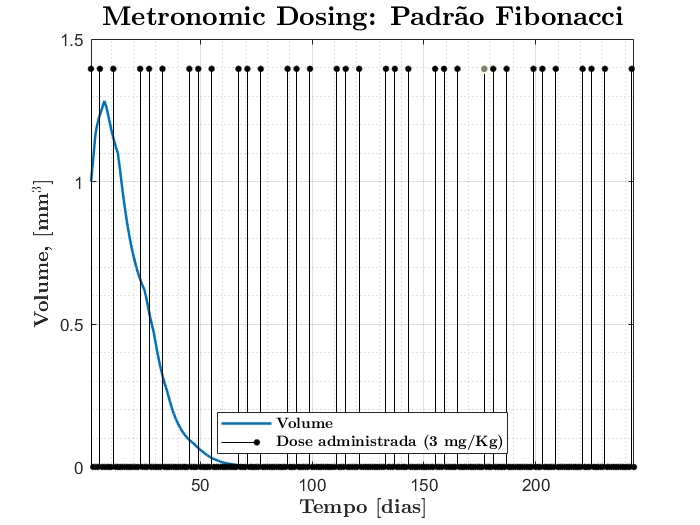
\includegraphics[width=0.5\textwidth]{img/perguntas/P5/P5-pattern.png}
    \begin{minipage}{2\linewidth}
        \caption{Sim. da administração mediante o 5º e 6º elemento da sequência, com \textit{rest period} = $10$d.}
        \label{fig:P5-pattern}
    \end{minipage}
\end{wrapfigure}

\vspace{-1.25em}
\begin{quote}
    \textit{``A general chemotherapeutic dosing regimen involves delivering a fixed pattern of equal doses, separated by ``rest periods'' \underline{to allow stemcell recovery}.''}\cite{Hahnfeldt2003-oy}
\end{quote}

A administração metronómica cíclica (\textit{metronomic pattern dosing}) evidencia uma regressão de volume tumoral menos célere que a observada no espaçamento \textit{Front-Load}, mantendo, no entanto, um baixo volume de forma contínua ao longo do tempo.

%//==============================--ii-==============================//%
%\vspace{-1.5em}
\paragraph{ii) \textit{Response to uneven vs. metronomic dosing}}\mbox{}\\
\vspace{-2em}
\label{subsubsubsec:amplitude-variation}
\begin{figure}[ht] 
    \begin{subfigure}[b]{0.5\linewidth}
        \centering
        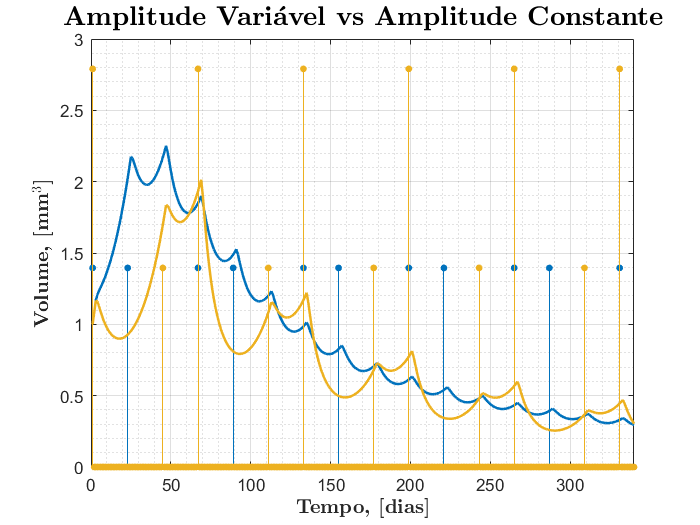
\includegraphics[width=0.8\linewidth]{img/perguntas/P5/P5-AmpVriation.png}
        \caption{Dose constante = 3 mg/kg a \textcolor{blue}{azul};\\ dose variável = 6 mg/kg, 0, 3 mg/kg periódicos a \textcolor{yellow}{amarelo}.} 
        \label{fig:AmpVarMatlab} 
        %\vspace{1ex}
    \end{subfigure}%% 
    \begin{subfigure}[b]{0.5\linewidth}
        \centering
        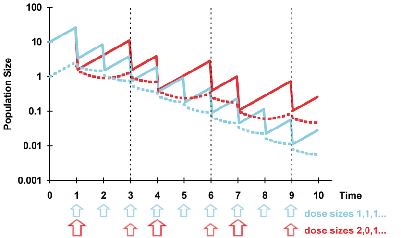
\includegraphics[width=0.8\linewidth]{img/perguntas/P5/P5-AmpVarDoc.png} 
        \caption{Dose constante = 1 mg/kg a \textcolor{blue}{azul};\\ dose variável = 2 mg/kg, 0, 1 mg/kg periódicos a \textcolor{red}{vermelho}.} 
        \label{fig:AmpVarDoc} 
        %\vspace{1ex}
    \end{subfigure}
    \vspace{-1.0em}\begin{minipage}{1\linewidth}
        \caption{Comparação entre espaçamentos constantes de dose variável e dose e permanente}
    \end{minipage}
\end{figure}

Tomando a abordagem metronómica como vetor de ataque preferível face à \hyperref[subsubsec:front-load-dosing]{\textit{Front-Load dosing}}, podemos ainda recorrer à comparação de uma administração equiespaçada no tempo de amplitude variável e metronómica de amplitude constante:
\vspace{-0.8em}
\begin{itemize}
    \item[$\rightarrow$] \textit{``Although the more up-front [amplitude variável] schedule is competitive early on, metronomic delivery provides better long-term suppression''}\cite{Hahnfeldt2003-oy} comprovada pela estabilidade da diminuição de volume \hyperref[fig:AmpVarDoc]{Fig. 11 (b)} a amplitudes constante e corroborada pela evolução observada na \hyperref[fig:AmpVarDoc]{Fig. 11 (a)}.
\end{itemize}

\noindent\textbf{Nota} $\rightarrow$ Vale salientar as regressões a pontilhado na \hyperref[fig:AmpVarDoc]{Fig. 11} representantes da evolução das células resistentes. É corroborado (através de simulações) o mencionado na \hyperref[subsubsec:metronomic-dosing]{secção anterior}: \textbf{o espaçamento metronómico controla o aumento de células resistentes}.
%//==============================--@--==============================//%
        \clearpage
%//==============================--@--==============================//%
\vspace{-1em}
\subsection{P6 | Desenvolvimento de resistência nas células cancerígenas}
\label{subsec:P6}

O processo de modelação do desenvolvimento de resistência nas células cancerígenas é de natureza não trivial. A resistência adquirida afeta, mediante vários vetores de ataque, o \hyperref[subsec:P2]{modelo farmacodinâmico} (\textit{drug-concentration response}), e é inerentemente dependente do corpo hospedeiro:

\begin{quote}
    \textit{``Resistance to therapy results from host factors, such as poor
    absorption or rapid metabolism, or epigenetic alterations in the cancer cells.''}\cite{teles_2017}
\end{quote}

Consequentemente, desenvolveram-se dois modelos baseados na interação \textit{drug-receptor}, de nomes \textbf{"Antagónico Competitivo"} e \textbf{"Antagónico Não Competitivo"}, cuja descrição é sucintamente inframencionada:

\begin{figure}[ht] 
    \begin{subfigure}[b]{0.5\linewidth}
        \hfill
        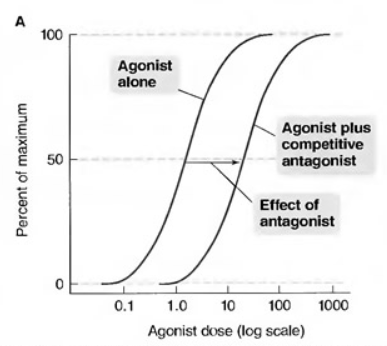
\includegraphics[width=0.8\linewidth]{img/perguntas/P6/P6-Competitive.png}
        \vspace{1ex}
        \hspace*{7.5em}\begin{minipage}{0.5\linewidth}
            \caption{Modelo competitivo} 
            \label{fig:LABEL-competitive} 
        \end{minipage}
    \end{subfigure}%% 
    \quad
    \begin{subfigure}[b]{0.5\linewidth}
        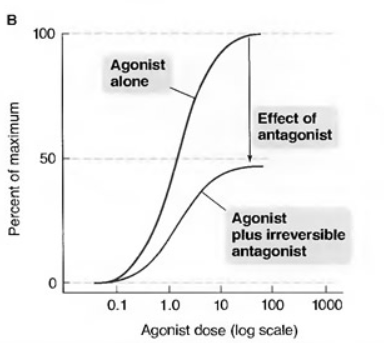
\includegraphics[width=0.8\linewidth]{img/perguntas/P6/P6-NCompetitive.png} 
        \vspace{1ex}
        \hspace*{3.5em}\begin{minipage}{0.5\linewidth}
            \caption{Modelo não competitivo} 
            \label{fig:LABEL-ncompetitive} 
        \end{minipage}
    \end{subfigure}
    \caption{\textit{Drug concentration-response} com efeito antagónico\cite{10.1093/bjaceaccp/mkh049}.}
\end{figure}

 \hyperref[fig:LABEL-competitive]{\textbf{A | Modelo Competitivo}}: A resistência compete com a ação do fármaco no recetor. O aumento de administração de fármaco detém o efeito da resistência (\textit{``(...) can be overcome by increasing the dose of the agonist [fármaco].''}\cite{10.1093/bjaceaccp/mkh049})
 
 \hspace*{1.25 em}\raisebox{0.2 em}{$\drsh$} \textbf{Efeito} $\rightarrow$ A curva \textit{drug-concentration response} sofre um desvio para a direita, mediante o incremento do parâmetro $C_{50}$.\footnotemark[9]

\begin{equation}
    \textbf{\hyperref[eq:modelo-PD]{Modelo de efeito (2)} adaptado} \rightarrow u \delequal \frac{C_p(t)}{(1 + r(t))\cdot C_{50} + C_p(t)}
\end{equation}

\hyperref[fig:LABEL-ncompetitive]{\textbf{B | Modelo não Competitivo}}: A resistência inibe a ação do fármaco no recetor. 
 
 \hspace*{1.25 em}\raisebox{0.2 em}{$\drsh$} \textbf{Efeito} $\rightarrow$ O efeito do fármaco é progressivamente menor, a curva de \textit{drug-concentration response} sofre um \textit{shrink}, \textit{``The actions of a non-competitive antagonist cannot be overcome by increasing the dose (...)''}.\cite{10.1093/bjaceaccp/mkh049}
 
\begin{equation}
    \textbf{\hyperref[eq:modelo-PD]{Modelo de efeito (2)} adaptado} \rightarrow u \delequal \frac{1}{1 + r(t)}\cdot\frac{C_p(t)}{C_{50} + C_p(t)}
\end{equation}

O modelo da resistência, $r(t)$, procura respresentar o efeito que baixas concentrações de fármaco induzem nas mutações das células cancerígenas. O modelo desenvolvido, bem como a sua representação gráfica encontram-se abaixo:
%//==============================--@--==============================//%
\footnotetext[9]{\textit{``Acquired resistance can be incorporated in the model by increasing the $C_{50}$ parameter from PD (...), since it will directly decrease the drug effect.''}\cite{teles_2017}}
%//==============================--@--==============================//%
\newpage
\begin{wrapfigure}{l}{0.5\textwidth}
    \centering
    \vspace{0.55 em}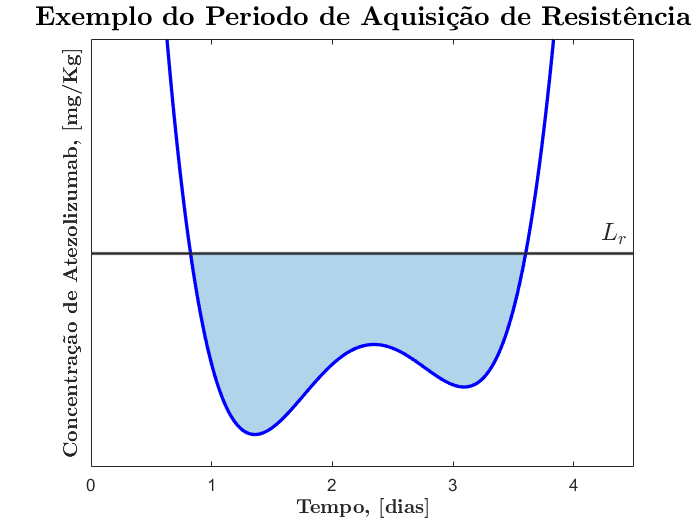
\includegraphics[width=0.5\textwidth]{img/perguntas/P6/P6-AreaMutation.png}
    \caption{Representação gráfica da área de desenvolvimento de resistência, a \textcolor{cyan}{azul}. A curva a \textcolor{blue}{azul escuro} representa uma curva de concentração.}
    \label{fig:P6-area}
\end{wrapfigure}

$$
    \xrightarrow[]{}
    \begin{cases}
        r(t) = K_r \cdot \int_{0}^{t} \max[0, L_r - C_p(\tau)] \,d\tau \\
        \dot{r}(t) = K_r \cdot \max[0, L_r - C_p(t)]
    \end{cases}
$$

Onde $K_r$ é o coeficiente de capacidade de mutação do tumor\cite{toxicity-lemos} e a resistência é apenas desenvolvida abaixo de uma linha de \textit{Threshold}, $L_r$ onde \textit{``(...) the driving tolerance is directly proportional to the intensities of past exposures (...)''}\cite{Porchet1988-bs} $\rightarrow$ cálculo da área de concentração abaixo do limite de \textit{Threshold}.

A simulação dos modelos foi realizada mediante um exemplo de terapia real de nome \textit{Intravenous (IV) Bolus Therapy}\footnotemark[10]\cite{teles_2017}:

\vphantom{Experiência 123}

\vphantom{Experiência 123}

\vspace{-2em}
\begin{figure}[ht]
    \begin{subfigure}[b]{0.5\linewidth}
        \centering
        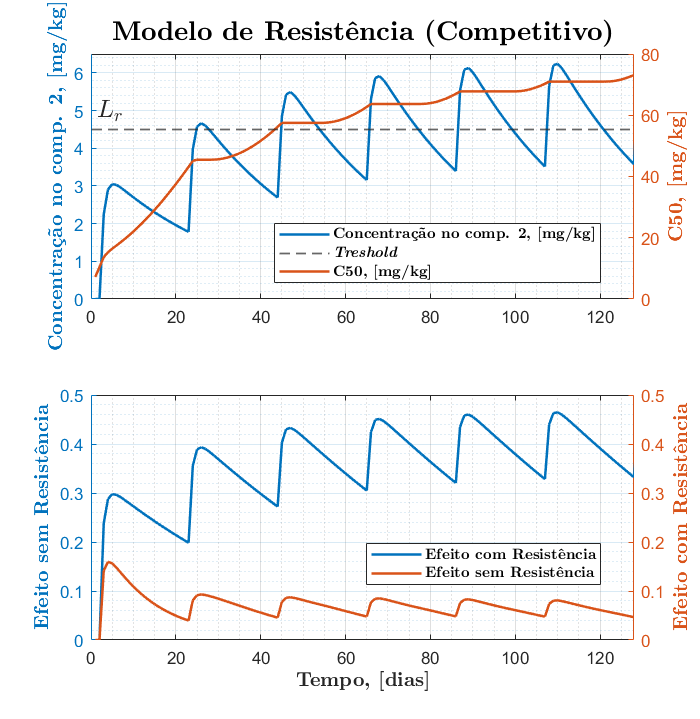
\includegraphics[width=0.9\linewidth]{img/perguntas/P6/P6-compete.png}
        \caption{Modelo de resistência antagonista competitiva.} 
        \label{fig:LABEL-compete} 
        %\vspace{1ex}
    \end{subfigure}%% 
    \begin{subfigure}[b]{0.5\linewidth}
        \centering
        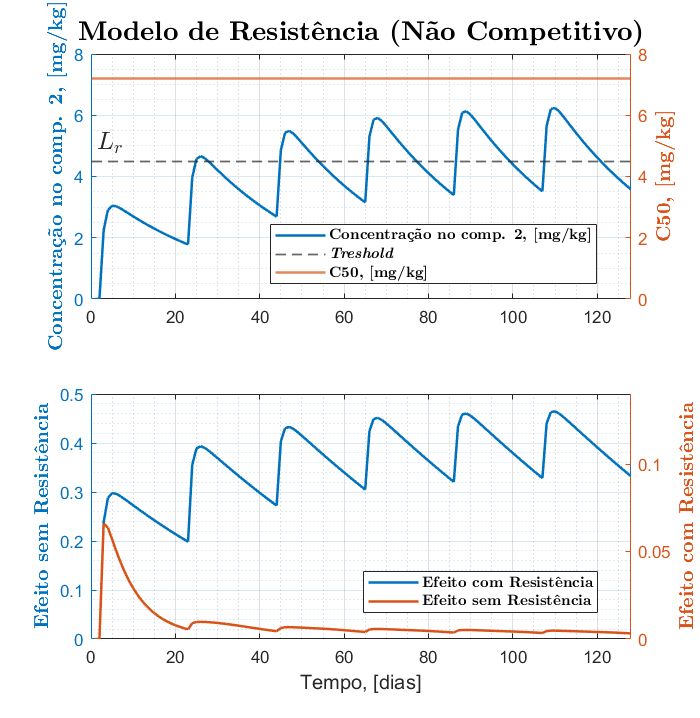
\includegraphics[width=0.9\linewidth]{img/perguntas/P6/P6-ncompete.png} 
        \caption{Modelo de resistência antagonista não competitiva.} 
        \label{fig:LABEL-ncompete} 
        %\vspace{1ex}
    \end{subfigure} 
    \caption{Concentração no compartimento de efeito ($C_p$), evolução do parâmetro $C_{50}$ e comparação dos efeitos sem resistência e com resistência para ambos os modelos para a terapia de parâmetros.}
\end{figure}

\vskip -0.5em

\textbf{(a)} $\rightarrow$ Para o modelo competitivo \textbf{o parâmetro $C_{50}$ incrementa apenas quando a concentração no compartimento de efeito é inferior à linha de \textit{Threshold}} (a integração em $r(t)$ é apenas realizada quando esta condição se verifica), de notar o \textbf{caráter oscilatório da regressão} (correspondente a iterações de incremento e estabilidade). \textbf{O efeito possui} \textbf{uma redução significativa} relativamente ao efeito não limitado pela resistência adquirida (consequência dos sucessivos desvios da curva de Hill).

\vskip 0.5em
\textbf{(b)} $\rightarrow$ Para o modelo não competitivo realça-se a \textbf{mitigação acentuada do efeito do fármaco}, quando comparado ao modelo anterior, coerente com o já discutido acima: Este modelo inibe o efeito, esta inibição não é solúvel por meio de incremento de concentração (\textbf{a curva de \textit{drug-concentration response}, sofre constrangimentos sucessivos, aproximando-se da nulidade)}.


%//==============================--@--==============================//%
\footnotetext[10]{$T = 21$d, dose $= 20$ mg/kg, para $K_r = 0.1$ e \textit{Threshold}$ = 4.5$}
%//==============================--@--==============================//%

\begin{wrapfigure}{l}{0.55\textwidth}
    \centering
    \vspace{-0.5 em}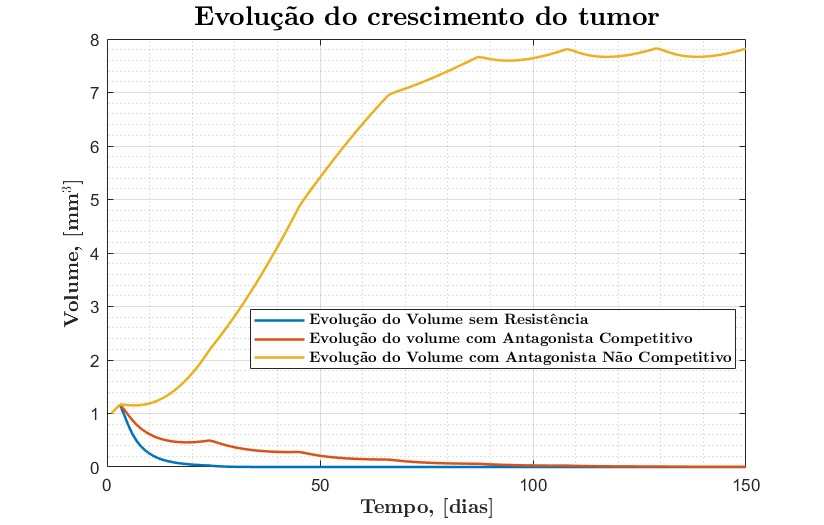
\includegraphics[width=0.55\textwidth]{img/perguntas/P6/P6-TumorGrowth.png}
    \caption{Comparação das 3 evoluções do tumor mediante o modelo de resistência projetado.}
    \label{fig:P6-volume}
\end{wrapfigure}

\vphantom{experiencia 123}
Supondo agora um \textit{Threshold} de 3.5, para o qual a concentração no compartimento de efeito é continuamente superior\footnotemark[11] (após algumas iterações de administração), duas conclusões são aparentes:

$\rightarrow$ A evolução do volume afetado pelo modelo antagonista competitivo é análoga à  evolução não afetada, possuindo apenas uma janela temporal mais alargada. Tal seria esperado: a resistência afeta a posição da curva de resposta do fármaco, mas não o seu \hyperref[eq:modelo-PD]{$u_{max}$}, $\pmb{\star}$ \textbf{a diminuição de volume é mais tardia}.

\vskip 0.5em

$\rightarrow$ A evolução do volume afetado pelo modelo antagonista não competitivo atinge um ponto de equilibrio, já discutido \hyperref[subsubsec:P3b]{secção P3}. Tal seria esperado: a resistência afeta o \hyperref[eq:modelo-PD]{$u_{max}$} da curva de resposta do fármaco, o seu efeito é sucessivamente e irreversivelmente menor.\\ $\pmb{\star}$ \textbf{Para mitigar este efeito seria necessário ser mais veloz que o desenvolvimento de resistência, o que equaciona em administrações iniciais de fármaco mais elevadas.}
%//==============================--@--==============================//%
\footnotetext[11]{O \textit{Threshold} previamente escolhido verificava-se sempre superior à concentração no compartimento de efeito de forma a demonstrar a evolução da atuação do fármaco. Em contexto real, supomos que a concentração de fármaco no corpo, após algumas administrações, consiga superar a criação de resistência. }

    %% refs
    %\clearpage
    \bibliographystyle{unsrtnat}
    \nocite{*}
    {\footnotesize%
    \bibliography{refs}}
    %% attachments
    %\newpage
    %\input{appendix.tex}

\end{document}
